\begin{example}
  Let us consider the polynomial ring $\mathbb{Q}[x, y, z]$ and
  the ideal $\{x*y - x, x^2 + x*z, y^2*z + x\}$. For this example we will
  use our implementation of the Mora and Robbiano algorithm.

  \begin{itemize}
  \item First we compute all the possible monomial orders. Enumerating all the possibilities
    these are the potential candidates:

    \begin{itemize}
    \item $\{(x*y) - x, (x^2) + x*z, (y^2*z) + x\}$
    \item $\{(x*y) - x, (x^2) + x*z, y^2*z + (x)\}$
    \item $\{(x*y) - x, x^2 + (x*z), (y^2*z) + x\}$
    \item $\{(x*y) - x, x^2 + (x*z), y^2*z + (x)\}$
    \item $\{x*y - (x), (x^2) + x*z, (y^2*z) + x\}$
    \item $\{x*y - (x), (x^2) + x*z, y^2*z + (x)\}$
    \item $\{x*y - (x), x^2 + (x*z), (y^2*z) + x\}$
    \item $\{x*y - (x), x^2 + (x*z), y^2*z + (x)\}$
    \end{itemize}

    However, not all the previous candidates will define monomial orders. Using a linear
    programming solver we obtain the following set of polynomials that define
    a monomial order:
    
    \begin{itemize}
    \item $\{(x*y) - x, (x^2) + x*z, (y^2*z) + x\}$
    \item $\{(x*y) - x, (x^2) + x*z, y^2*z + (x)\}$
    \item $\{(x*y) - x, x^2 + (x*z), (y^2*z) + x\}$
    \end{itemize}

  \item Now we extend each set of polynomials to marked \grob bases.
    We obtain:

    \begin{itemize}
    \item $\{(x*y) - x, x^2 + (x*z), (y^2*z) + x\}$
    \item $\{(x*y) - x, (x^2) + x*z, y^2*z + x, (-y^3*z) + y^2*z\}$
    \item $\{(x*y) - x, (x^2) + x*z, (y^2*z) + x\}$
    \end{itemize}

  \item Finally, we obtain the reduced marked \grob basis, this step help
    to eliminate marked \grob bases than define the same monomial order.
    In this case, we kept the same number of reduced marked \grob basis
    but we eliminated redundant polynomials:

    \begin{itemize}
    \item $\{(x^2) + x*z, (x*y) - x, (y^2*z) + x\}$ 
    \item $\{(-y^3*z) + y^2*z, y^2*z + (x)\}$  
    \item $\{x^2 + (x*z), (x*y) - x, (y^2*z) + x\}$
    \end{itemize}
  \end{itemize}
  
  \begin{figure}[h]
    \centering
    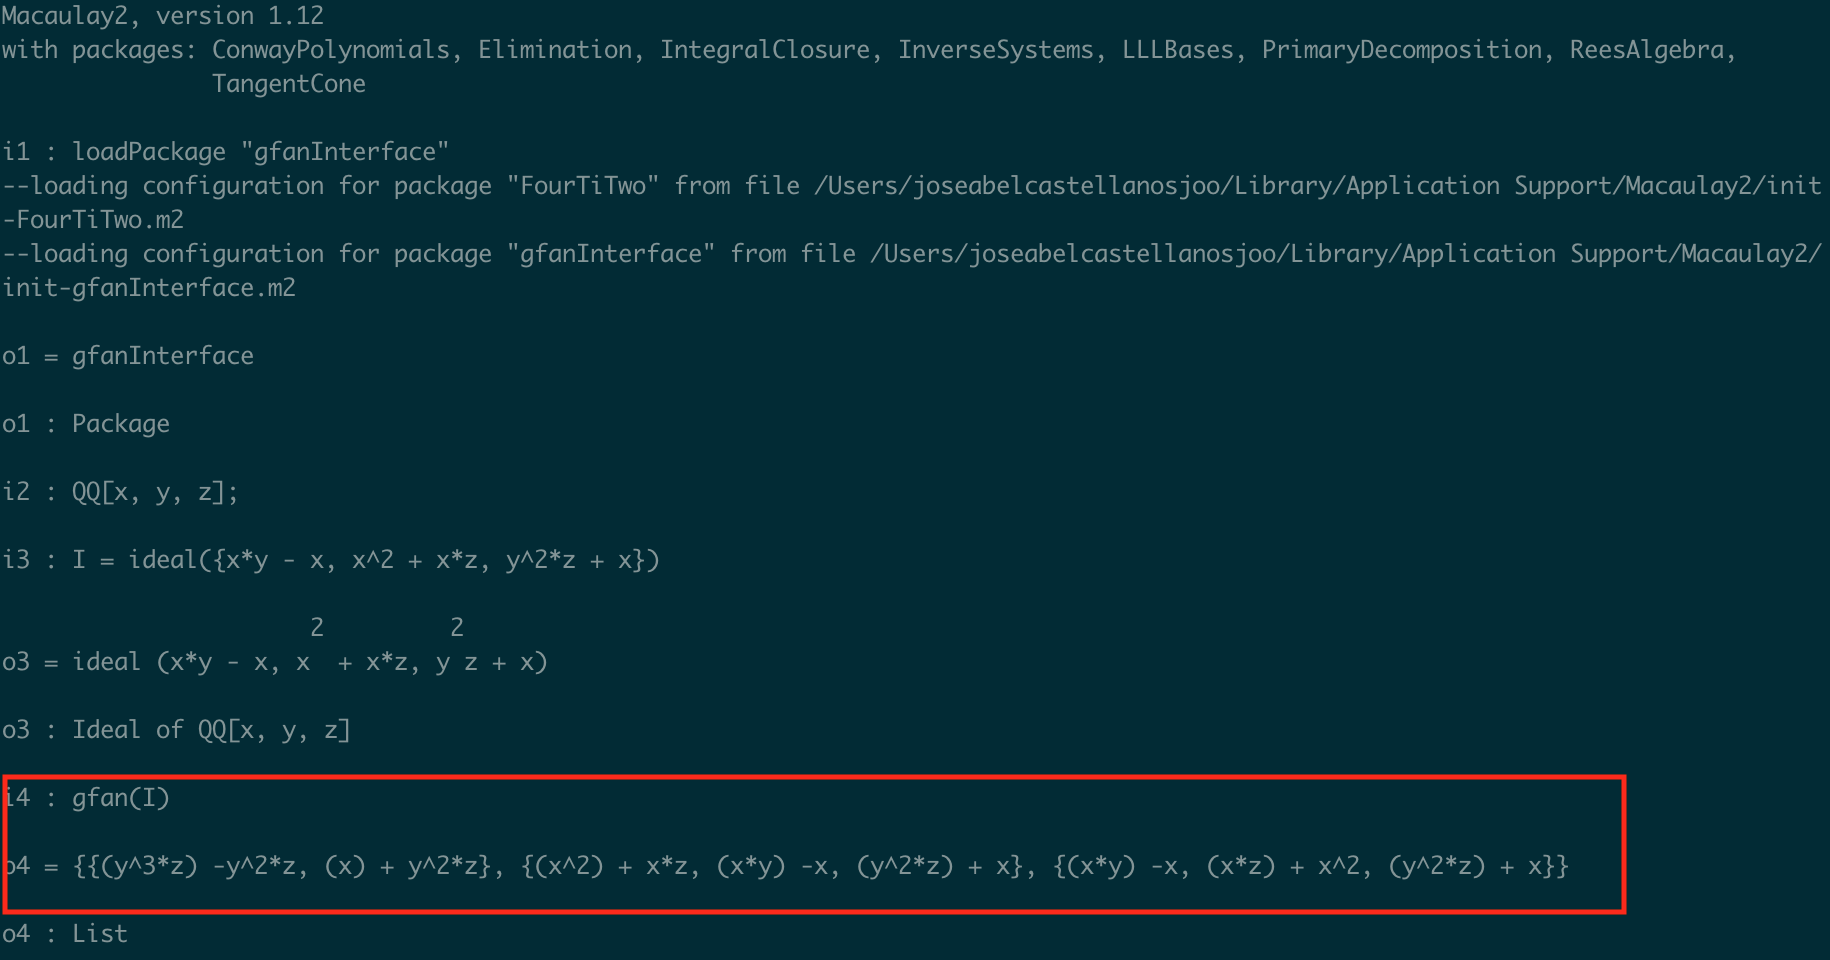
\includegraphics[width=9cm]{gfanIdeal3}
    
\includegraphics[width=6cm]{ideal3}
    \caption{(Left) Using gfan to compute the \grob fan of the ideal
      $\{x*y - x, x^2 + x*z, y^2*z + x\}$; (Right) Visualization of the \grob
    fan of the ideal $\{x*y - x, x^2 + x*z, y^2*z + x\}$}
  \end{figure}
\end{example}

%%% Local Variables:
%%% mode: latex
%%% TeX-master: "main"
%%% End:
